\section{Gauss-Legendre Method for Computing the Integral}
\label{sec:GaussLegendreMethod}

To be able to use the Gauss-Legendre method to compute the integral in \matref{eq:NatureOfTheProblem2}, the limits of the integral must be made  finite.
Since the wave function 
\begin{align}
	e^{-2\alpha x}
\end{align}
rapidly goes toward zero as $x$ is increased (see \figref{fig:function_zeropoint}), the integral can be approximated  by the same integral with finite limits.

\begin{figure}[H]
	\centering
	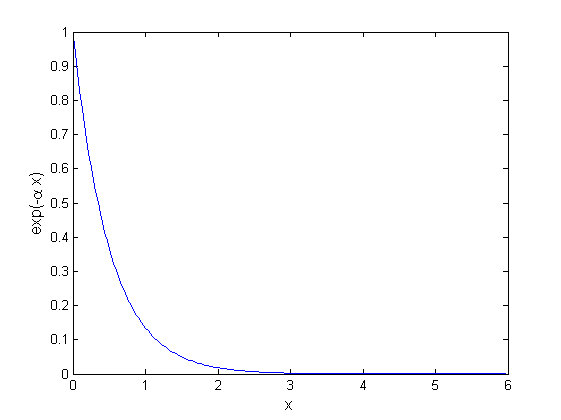
\includegraphics[width=0.75\textwidth]{Figures/function_zeropoint.png}
	\caption{Plot of $e^{-2\alpha x}$ with $\alpha = 2$.}
	\label{fig:function_zeropoint}
\end{figure}
In this project, if the value is equal or smaller than $10^{-6}$ it is close enough to zero to neglect contributions from the part of the wave function when the wave function gives a value of this order.
For $x=4$ the value of the wave function is $e^{-2\cdot \alpha \cdot 4} \approx 1.1\cdot 10^{-6}$, when $\alpha = 2$.
Hence, the considered integral that is to be solved by the Gauss-Legendre method is given by
\begin{align}
   \left< \frac{1}{| \v{r}_1 - \v{r}_2 |} \right> 
   = \int _{-4} ^{4} \frac{e^{-2\alpha (r_1+r_2)}}{| \v{r}_1 - \v{r}_2 |} d \v{r}_1 d\v{r}_2
\label{eq:GLdMethod1}
\end{align} 
To be able to use the Gauss-Legendre method, the limits have to be $-1$ and $1$. 
This is, however, easily obtained by a change in variables using the following quantity
\begin{align}
	\int _a ^b f(t) dt = \int _{-1} ^1 f \left( \frac{b-a}{2} x + \frac{b+a}{2} \right) dx
	\label{eq:GLdMethod2}
\end{align} 
The first step of the Gauss-Legendre method is then to compute the roots of the $n$'th Legendre polynomial.
The $i$'th root $z_i$ is approximated by
\begin{align}
	z_i = \cos \left( \frac{\pi (4\cdot i - 1)}{4n+2} \right)
	\label{eq:GLdMethod3}
\end{align} 
for large $n$.
The $n$'th Legendre polynomial $L_n(x)$ can then be computed using the recursive relation
\begin{align}
	(j+1)L_{j+1} (z) + j L_{j-1} (x) -(2j+1) z L_j (z) = 0
	\label{eq:GLdMethod4}
\end{align} 
with $L_{-1} (x) = 0$ and $L_0 (x) = 1$.
The code for generation the Legendre polynomial can be found in \secref{sec:GenerationOfLegendrePolynomials} together with a test of the Legendre polynomial generating algorithm.

The derivative of the Legendre polynomial can then be computed as
\begin{align}
	L_n '(z) = \frac{-n\cdot z \cdot L_n (z) +n \cdot L_{n-1} (z)}{1-z^2} 
	\label{eq:GLdMethod4a}
\end{align}

Newton's method is then applied to find the best estimation of the roots by considering the expression
\begin{align}
	z_1 = z- \frac{L_n(z)}{L_n'(z)}
	\label{eq:GLdMethod5}
\end{align}
in which $z$ is the first approximation of the root given by \matref{eq:GLdMethod3}, and $z_1$ is a better approximation for the root. 
The algorithm for generation of the roots and the Legendre polynomials is run until the difference between $z_1$ and the root approximated by \matref{eq:GLdMethod3} is ultimately zero, which in this project is set to $10^{-6}$.

The weight $w_i$ of the $i$'th root $z_i$ is then obtained by
\begin{align}
	w_i = \frac{2}{(1-z_i^2)(L_n'(z_i))^2}
	\label{eq:GLdMethod6}
\end{align}
  

